%!Mode:: "TeX:UTF-8"
\section{栈溢出和堆溢出}

A thread's assigned stack size can be as small as a few dozen kilobytes. Allocating more memory on the stack than is available can result in a crash due to stack overflow.

\begin{figure}[ht]
	\begin{center}
		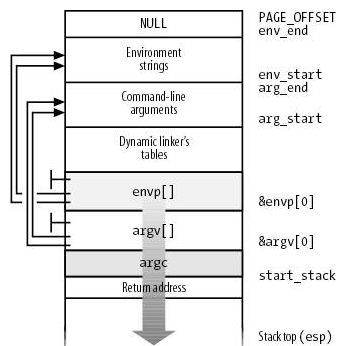
\includegraphics[keepaspectratio,width=0.3\paperwidth]{Pictures/LinuxUserStack.png}
	\caption{用户栈顶端}
	\label{fig:LinuxUserStack}
	\end{center}
\end{figure}

栈和堆溢出的一个共性就是第三方可以完全依靠提供特定数据实现代码级别的入侵。
堆溢出执行恶意代码的一种情况是通过过长的数据破坏堆管理记录结构,使下次申请能得到保存某些特定函数指针的位置,然后进行修改。
此外,由于字符串处理函数(gets,strcpy等等)没有对数组越界加以监视和限制,我们利用字符数组写越界,覆盖堆栈中的老元素的值,就可以修改返回地址。 

gets函数(\verb$char *gets(char *s);$)和fgets(\verb$char *fgets(char*, int, FILE*);$)函数最大的不同是gets函数的缓冲区虽然由用户提供,但是用户无法指定其一次最多读入多少字节的内容。这一点导致gets变成了一个非常危险的函数。

有时,堆和栈的溢出分别指内存空间的耗尽。
递归可能会导致栈耗尽,内存泄露会导致堆耗尽。
 
\clearpage